\documentclass[12pt,a4paper]{article}

% Packages
\usepackage[utf8]{inputenc}
\usepackage[T1]{fontenc}
\usepackage{lmodern}
\usepackage[margin=1in,headheight=15pt]{geometry}
\usepackage{graphicx}
\usepackage{tikz}
\usetikzlibrary{shapes.geometric, arrows.meta, positioning, fit, backgrounds, calc}
\usepackage{listings}
\usepackage{xcolor}
\usepackage{hyperref}
\usepackage{booktabs}
\usepackage{float}
\usepackage{caption}
\usepackage{subcaption}
\usepackage{amsmath}
\usepackage{enumitem}
\usepackage{fancyhdr}
\usepackage{titlesec}

% Colors
\definecolor{codegreen}{rgb}{0,0.6,0}
\definecolor{codegray}{rgb}{0.5,0.5,0.5}
\definecolor{codepurple}{rgb}{0.58,0,0.82}
\definecolor{backcolour}{rgb}{0.95,0.95,0.92}
\definecolor{meluxinaBlue}{RGB}{0,102,179}
\definecolor{serverGreen}{RGB}{76,175,80}
\definecolor{clientOrange}{RGB}{255,152,0}
\definecolor{monitorPurple}{RGB}{156,39,176}
\definecolor{discoveryTeal}{RGB}{0,150,136}

% Code listing style
\lstdefinestyle{mystyle}{
    backgroundcolor=\color{backcolour},   
    commentstyle=\color{codegreen},
    keywordstyle=\color{magenta},
    numberstyle=\tiny\color{codegray},
    stringstyle=\color{codepurple},
    basicstyle=\ttfamily\footnotesize,
    breakatwhitespace=false,         
    breaklines=true,                 
    captionpos=b,                    
    keepspaces=true,                 
    numbers=left,                    
    numbersep=5pt,                  
    showspaces=false,                
    showstringspaces=false,
    showtabs=false,                  
    tabsize=2
}
\lstset{style=mystyle}

% YAML language definition
\lstdefinelanguage{yaml}{
    keywords={true,false,null,y,n},
    sensitive=false,
    comment=[l]{\#},
    morestring=[b]',
    morestring=[b]"
}

% JSON language definition
\lstdefinelanguage{json}{
    string=[s]{"}{"}, 
    comment=[l]{//},
    morecomment=[s]{/*}{*/},
    literate=
     *{0}{{{\color{blue}0}}}{1}
      {1}{{{\color{blue}1}}}{1}
      {2}{{{\color{blue}2}}}{1}
      {3}{{{\color{blue}3}}}{1}
      {4}{{{\color{blue}4}}}{1}
      {5}{{{\color{blue}5}}}{1}
      {6}{{{\color{blue}6}}}{1}
      {7}{{{\color{blue}7}}}{1}
      {8}{{{\color{blue}8}}}{1}
      {9}{{{\color{blue}9}}}{1}
}

% Header/Footer
\pagestyle{fancy}
\fancyhf{}
\rhead{AI-Factories Framework}
\lhead{EUMaster4HPC Student Challenge 2025}
\rfoot{Page \thepage}

% Hyperref setup
\hypersetup{
    colorlinks=true,
    linkcolor=meluxinaBlue,
    filecolor=magenta,      
    urlcolor=cyan,
    pdftitle={Benchmarking AI Factories on MeluXina Supercomputer},
}

\title{
    \vspace{-1cm}
    \textbf{Benchmarking AI Factories on MeluXina Supercomputer}\\
    \large A Unified Platform for Deploying, Monitoring, and Benchmarking\\
    AI Factories\\
    \vspace{0.5cm}
    \normalsize EUMaster4HPC Student Challenge 2025
}

\author{
    Tommaso Crippa\\
    Edoardo Leali\\
    Emanuele Caruso
}

\date{12 January 2026}

\begin{document}

\maketitle

\begin{abstract}
This report presents our implementation for the EUMaster4HPC Student Challenge 2025, where we were tasked to build a unified framework designed to streamline the deployment, monitoring, and benchmarking of AI inference services on High-Performance Computing clusters. The framework addresses the challenges of managing containerized AI workloads in SLURM-based environments. AI-Factories provides three integrated modules (Server, Monitor, and Client) that work together through an automatic service discovery mechanism. The framework enables researchers and engineers to deploy inference servers, monitor performance metrics via Prometheus, and execute standardized benchmarks with minimal manual configuration. This report details the system architecture, design decisions, implementation specifics, and provides guidance on deploying the framework on the MeluXina supercomputer.
\end{abstract}

\tableofcontents
\newpage

%==============================================================================
\section{Introduction}
%==============================================================================

\subsection{The Rise of AI Factories}

The artificial intelligence landscape is undergoing a fundamental transformation with the emergence of AI Factories, large-scale inference platforms designed to serve AI models at production scale. Unlike traditional research-focused deployments, AI Factories represent the industrialization of AI, where models must deliver consistent, low-latency responses to thousands of concurrent users while maintaining cost efficiency and reliability.

This shift from experimentation to production has been driven by multiple interconnected factors. The explosion of \textbf{foundation models}, including large language models, vision models, and multimodal systems, has created unprecedented demand for specialized inference infrastructure capable of handling production workloads. Organizations across industries are moving beyond proof-of-concept deployments and adopting AI as \textbf{mission-critical technology}, requiring robust infrastructure with enterprise-grade reliability. The \textbf{scale requirements} have grown dramatically, with single inference endpoints now expected to serve millions of requests daily. At the same time, there is mounting pressure to optimize \textbf{GPU utilization} and reduce inference costs, as infrastructure budgets become increasingly constrained. These factors combined have transformed AI from a research curiosity into a production engineering problem.

\subsection{Why HPC Clusters Need Better Benchmarking}

HPC clusters are a perfect fit for AI Factories, but they are not used enough. Cloud providers dominate AI inference today, yet HPC systems have clear benefits. \textbf{GPU accelerators} such as NVIDIA A100 and H100 provide state-of-the-art performance with fast interconnections between nodes. \textbf{University infrastructure} eliminates the hourly charges typical of cloud services, making long-term deployments more economical. Inference workloads can run close to training data and other research activities, reducing data movement and latency. Most importantly, \textbf{SLURM} provides precise control over CPU, memory, and GPU allocation, allowing researchers to optimize resource usage for their specific needs.

However, using HPC for AI Factories creates problems that cloud platforms do not have. \textbf{SLURM complexity} arises from running inference services as batch jobs instead of traditional always-on containerized deployments. \textbf{Dynamic allocation} means services are assigned to different compute nodes each time a job is submitted. There is no built-in DNS or load balancing mechanism for dynamically allocated services, forcing users to manually track endpoints. \textbf{Monitoring tools} like Prometheus were designed for static cloud environments and do not naturally handle ephemeral HPC jobs. Additionally, \textbf{Apptainer} security models differ fundamentally from Docker and Kubernetes paradigms, requiring different approaches to container management and resource isolation.

Current benchmarking tools do not work well for HPC. They have three fundamental problems. First, \textbf{cloud-centric tooling} such as Locust, K6, and wrk expect fixed HTTP endpoints and do not integrate with SLURM schedulers. These tools cannot handle the dynamic nature of HPC job allocation or coordinate monitoring across temporary compute nodes that are created and destroyed with each job submission. Second, the current approach requires \textbf{manual setup processes} including copying job IDs, extracting node names, and configuring Prometheus targets. These error-prone steps introduce variability and make results unreliable, causing a \textbf{reproducibility crisis} where most published benchmarks cannot be repeated by other researchers due to undocumented configuration details. Third, \textbf{incomplete metrics} focus exclusively on latency and throughput but ignore HPC-specific concerns such as GPU cache utilization, memory bandwidth saturation, scheduler overhead, and multi-tenant interference from other users. Without these specialized metrics, researchers cannot effectively optimize inference workloads for HPC characteristics and cannot understand how their systems perform under realistic production conditions.

HPC-based AI Factories need a unified framework that simplifies SLURM integration while preserving access to important HPC features. The framework must provide automatic service discovery in dynamic environments where node assignments change with each deployment. It should collect HPC-specific monitoring metrics beyond standard cloud benchmarks. The system must make benchmarks reproducible through declarative configuration files that can be version-controlled and shared among researchers. Finally, it needs to bridge the gap between cloud AI tools and HPC infrastructure, bringing modern AI development practices to supercomputers while respecting the unique constraints and opportunities that HPC environments offer.

\subsection{Project Goals}

AI-Factories was developed to meet several key objectives. The framework provides a \textbf{unified command-line interface} that handles server deployment, monitoring, and benchmarking through a single consistent tool. It \textbf{eliminates manual endpoint management} through automatic service discovery, removing the need to manually track and configure service addresses. The system enables \textbf{recipe-based configuration} that makes deployments reproducible and shareable across teams. It fully \textbf{supports GPU-accelerated inference servers} on HPC clusters, taking advantage of supercomputer hardware for AI workloads. \textbf{Prometheus monitoring is integrated} with automatic target resolution, so that metric collection is set up without manual configuration. Finally, the framework \textbf{facilitates performance benchmarking} with configurable workload patterns, allowing researchers to test their systems under diverse conditions.

\subsection{Target Platform: MeluXina}

MeluXina is Luxembourg's national supercomputer, featuring AMD EPYC processors and NVIDIA A100 GPUs. The framework is specifically designed to work with the \textbf{SLURM workload manager} for job scheduling, which is the standard scheduler on HPC systems. It uses \textbf{Apptainer} (formerly Singularity) for secure containerization of inference workloads. The system integrates with the \textbf{module system} for managing software environments across different compute nodes. Finally, it takes advantage of \textbf{shared scratch storage} available on supercomputers for storing container images and benchmark data.

%==============================================================================
\section{System Architecture}
%==============================================================================

The AI-Factories framework follows a modular architecture with three core modules and a central service discovery mechanism. Figure~\ref{fig:architecture} illustrates the high-level system design.

\begin{figure}[H]
\centering
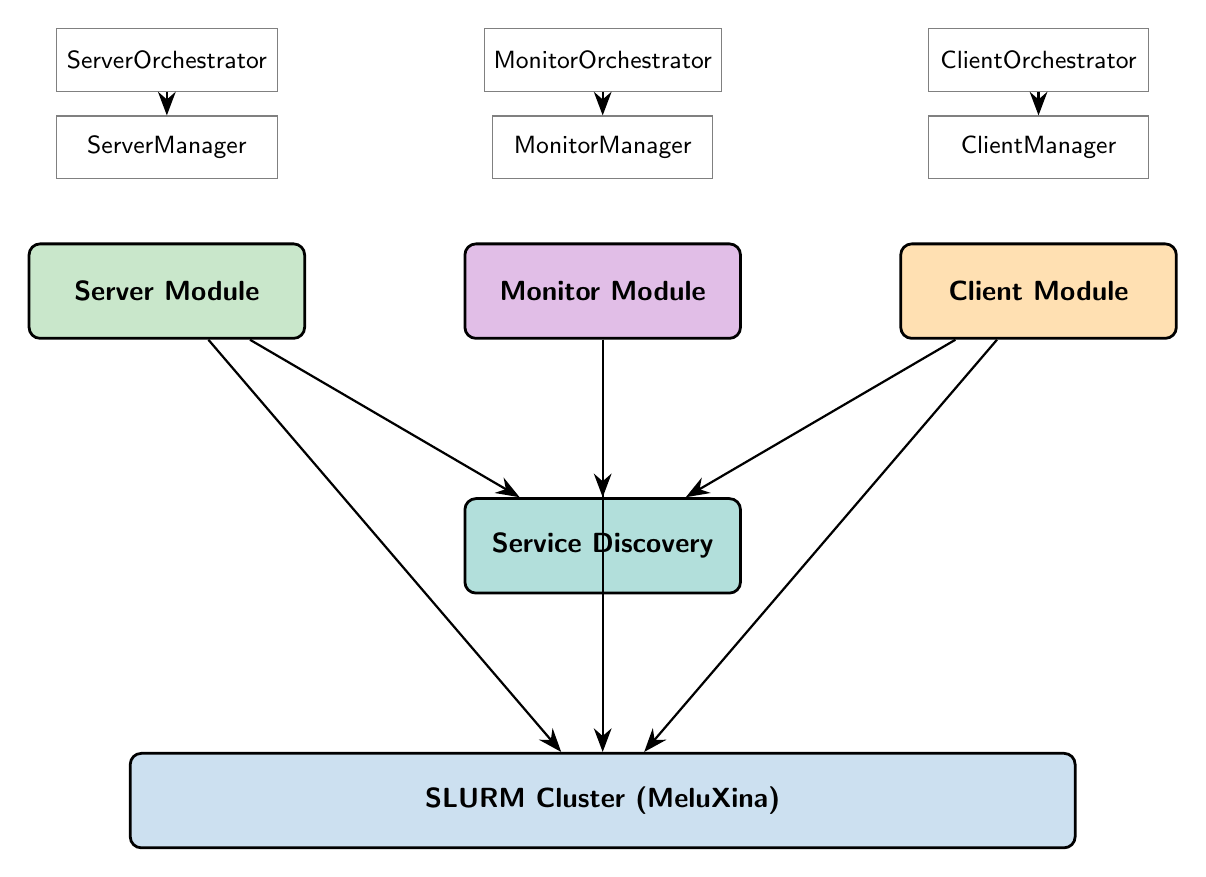
\begin{tikzpicture}[
    node distance=1.5cm and 2cm,
    module/.style={rectangle, rounded corners, draw=black, line width=1pt, minimum width=3.5cm, minimum height=1.2cm, font=\sffamily\bfseries},
    component/.style={rectangle, draw=gray, fill=white, minimum width=2.8cm, minimum height=0.8cm, font=\sffamily\small},
    arrow/.style={-{Stealth[length=3mm]}, thick},
    dasharrow/.style={-{Stealth[length=3mm]}, thick, dashed}
]

% Core Modules
\node[module, fill=serverGreen!30] (server) {Server Module};
\node[module, fill=monitorPurple!30, right=of server] (monitor) {Monitor Module};
\node[module, fill=clientOrange!30, right=of monitor] (client) {Client Module};

% Service Discovery
\node[module, fill=discoveryTeal!30, below=2cm of monitor] (discovery) {Service Discovery};

% SLURM Layer
\node[module, fill=meluxinaBlue!20, below=2cm of discovery, minimum width=12cm] (slurm) {SLURM Cluster (MeluXina)};

% Components under each module
\node[component, above=0.8cm of server] (sm) {ServerManager};
\node[component, above=0.3cm of sm] (so) {ServerOrchestrator};

\node[component, above=0.8cm of monitor] (mm) {MonitorManager};
\node[component, above=0.3cm of mm] (mo) {MonitorOrchestrator};

\node[component, above=0.8cm of client] (cm) {ClientManager};
\node[component, above=0.3cm of cm] (co) {ClientOrchestrator};

% Arrows
\draw[arrow] (server) -- (discovery);
\draw[arrow] (monitor) -- (discovery);
\draw[arrow] (client) -- (discovery);

\draw[arrow] (server) -- (slurm);
\draw[arrow] (monitor) -- (slurm);
\draw[arrow] (client) -- (slurm);

\draw[dasharrow] (so) -- (sm);
\draw[dasharrow] (mo) -- (mm);
\draw[dasharrow] (co) -- (cm);

\end{tikzpicture}
\caption{AI-Factories High-Level Architecture}
\label{fig:architecture}
\end{figure}

\subsection{Architectural Principles}

The framework is built on several key architectural principles that guide its design and implementation. \textbf{Separation of Concerns} ensures that each module handles a specific domain (deployment, monitoring, benchmarking) with clear interfaces, making the codebase maintainable and easier to extend. \textbf{Recipe-Based Configuration} means that all operations are driven by YAML recipes rather than imperative code, enabling reproducibility and version control of deployments. The \textbf{Manager-Orchestrator Pattern} is used throughout the framework, where each module has a Manager class that handles business logic and an Orchestrator class that interacts directly with SLURM, providing clean separation between domain logic and infrastructure details. \textbf{Automatic Discovery} allows services to register their endpoints automatically as they deploy, eliminating manual configuration propagation and reducing operational overhead.

\subsection{Directory Structure}

The framework organizes code and configuration as follows:

\begin{lstlisting}[language=bash, caption={Project Directory Structure}]
AI-Factories/
|-- src/
|   |-- server/          # Server deployment module
|   |-- monitor/         # Prometheus monitoring module
|   |-- client/          # Benchmark client module
|   |-- discover.py      # Service discovery mechanism
|   |-- list_services.py # CLI for listing services
|   +-- clear_services.py
|-- recipes/
|   |-- servers/         # Server deployment recipes
|   |-- monitors/        # Monitor configuration recipes
|   +-- clients/         # Benchmark workload recipes
|-- config/
|   +-- slurm.yml        # SLURM configuration defaults
|-- logs/                # Runtime logs and state
+-- results/             # Benchmark output files
\end{lstlisting}

%==============================================================================
\section{Service Discovery Mechanism}
%==============================================================================

One of the key innovations in AI-Factories is the automatic service discovery system. This mechanism solves the fundamental challenge of dynamic endpoint management in SLURM environments.

\subsection{The Discovery Problem}

When submitting jobs to SLURM, the scheduler assigns compute nodes dynamically. This creates a challenge: how do clients and monitors find the server they need to connect to? Traditional approaches require:

\begin{enumerate}
    \item Waiting for job allocation
    \item Querying SLURM for the assigned node
    \item Manually copying the endpoint to other configurations
\end{enumerate}

\subsection{Solution: File-Based Service Registry}

AI-Factories implements a lightweight, file-based service registry stored in the user's home directory:

\begin{lstlisting}[language=bash]
~/.aibenchmark/discover/
|-- vllm.json
|-- ollama.json
+-- chromadb.json
\end{lstlisting}

Each service file contains the connection information:

\begin{lstlisting}[language=json, caption={Discovery File Format}]
{
  "job_id": "3757043",
  "recipe_name": "vllm-server",
  "instance_id": "a1b2c3d4-...",
  "node": "mel2013",
  "ports": [8000]
}
\end{lstlisting}

\subsection{Discovery Workflow}

Figure~\ref{fig:discovery} shows the discovery workflow in action.

\begin{figure}[H]
\centering
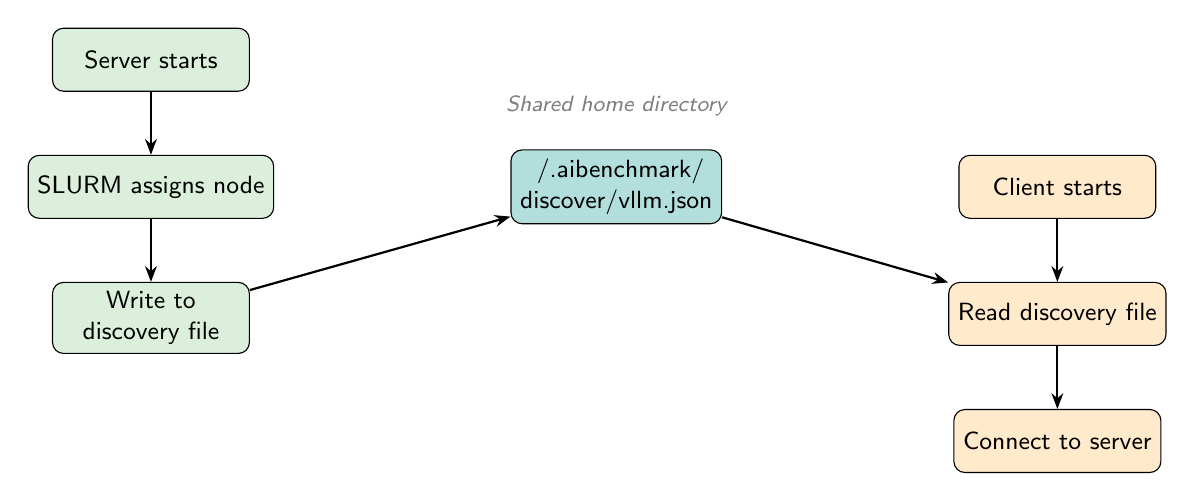
\begin{tikzpicture}[
    node distance=0.8cm,
    block/.style={rectangle, draw, rounded corners, minimum width=2.5cm, minimum height=0.8cm, font=\sffamily\small, align=center},
    arrow/.style={-{Stealth[length=2mm]}, thick},
    note/.style={font=\sffamily\footnotesize\itshape, text=gray}
]

% Server side
\node[block, fill=serverGreen!20] (s1) {Server starts};
\node[block, fill=serverGreen!20, below=of s1] (s2) {SLURM assigns node};
\node[block, fill=serverGreen!20, below=of s2] (s3) {Write to\\discovery file};

% Discovery file
\node[block, fill=discoveryTeal!30, right=3cm of s2] (disc) {~/.aibenchmark/\\discover/vllm.json};

% Client side
\node[block, fill=clientOrange!20, right=3cm of disc] (c1) {Client starts};
\node[block, fill=clientOrange!20, below=of c1] (c2) {Read discovery file};
\node[block, fill=clientOrange!20, below=of c2] (c3) {Connect to server};

% Arrows
\draw[arrow] (s1) -- (s2);
\draw[arrow] (s2) -- (s3);
\draw[arrow] (s3) -- (disc);
\draw[arrow] (c1) -- (c2);
\draw[arrow] (disc) -- (c2);
\draw[arrow] (c2) -- (c3);

% Notes
\node[note, above=0.3cm of disc] {Shared home directory};

\end{tikzpicture}
\caption{Service Discovery Workflow}
\label{fig:discovery}
\end{figure}

\subsection{Service Name Linking}

All recipes for the same service share a common \texttt{service\_name} field:

\begin{lstlisting}[language=yaml, caption={Service Name Consistency Across Recipes}]
# recipes/servers/vllm-server.yaml
name: vllm-server
service_name: vllm  # Discovery key

# recipes/monitors/vllm-monitor.yml
name: vllm-monitor
service_name: vllm  # Same key

# recipes/clients/vllm-simple-test.yaml
name: vllm-simple-test
service_name: vllm  # Same key
\end{lstlisting}

This design allows the client and monitor to automatically find the server without any manual endpoint configuration.

%==============================================================================
\section{Server Module}
%==============================================================================

The Server Module is responsible for deploying AI inference services as SLURM jobs using containerized applications.

\subsection{Module Architecture}

\begin{figure}[H]
\centering
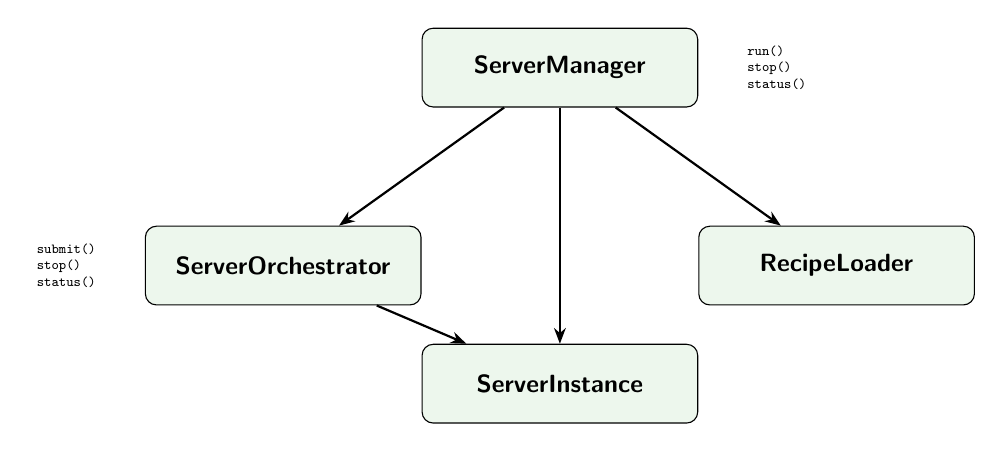
\begin{tikzpicture}[
    node distance=1cm and 1.5cm,
    class/.style={rectangle, draw, rounded corners, fill=serverGreen!10, minimum width=3.5cm, minimum height=1cm, font=\sffamily\small},
    method/.style={font=\ttfamily\tiny, align=left},
    arrow/.style={-{Stealth[length=2mm]}, thick}
]

\node[class] (manager) {\textbf{ServerManager}};
\node[class, below left=1.5cm and 0cm of manager] (orchestrator) {\textbf{ServerOrchestrator}};
\node[class, below right=1.5cm and 0cm of manager] (loader) {\textbf{RecipeLoader}};
\node[class, below=3cm of manager] (instance) {\textbf{ServerInstance}};

\draw[arrow] (manager) -- (orchestrator);
\draw[arrow] (manager) -- (loader);
\draw[arrow] (manager) -- (instance);
\draw[arrow] (orchestrator) -- (instance);

% Methods
\node[method, right=0.5cm of manager] {
    run()\\
    stop()\\
    status()
};

\node[method, left=0.5cm of orchestrator] {
    submit()\\
    stop()\\
    status()
};

\end{tikzpicture}
\caption{Server Module Class Structure}
\label{fig:server-module}
\end{figure}

\subsubsection{ServerManager}

The \texttt{ServerManager} class serves as the primary interface for server operations. It coordinates recipe loading, job submission, and instance lifecycle management.

Key responsibilities:
\begin{itemize}
    \item Loading and validating server recipes
    \item Creating \texttt{ServerInstance} objects for each deployment
    \item Coordinating with the orchestrator for SLURM submissions
    \item Waiting for node assignment and updating discovery information
    \item Managing the collection of active server instances
\end{itemize}

\subsubsection{ServerOrchestrator}

The \texttt{ServerOrchestrator} handles direct interaction with SLURM:

\begin{itemize}
    \item Building SBATCH scripts from recipe specifications
    \item Submitting jobs using the \texttt{sbatch} command
    \item Querying job status with \texttt{squeue}
    \item Canceling jobs with \texttt{scancel}
\end{itemize}

The orchestrator generates batch scripts dynamically based on recipe resources:

\begin{lstlisting}[language=bash, caption={Generated SBATCH Script Structure}]
#!/bin/bash -l

#SBATCH --job-name=vllm-server_a1b2c3d4
#SBATCH --time=04:00:00
#SBATCH --partition=gpu
#SBATCH --account=p200981
#SBATCH --nodes=1
#SBATCH --cpus-per-task=8
#SBATCH --mem=64G
#SBATCH --gres=gpu:1

# Recipe-defined startup commands
module load Apptainer/1.3.6-GCCcore-13.3.0
apptainer exec $IMAGE python -m vllm.entrypoints.openai.api_server ...
\end{lstlisting}

\subsubsection{ServerInstance}

Each deployment creates a \texttt{ServerInstance} object tracking:
\begin{itemize}
    \item Unique instance identifier
    \item SLURM job ID (orchestrator handle)
    \item Current status (SUBMITTED, STARTING, RUNNING, etc.)
    \item Assigned node and ports
    \item Recipe reference
\end{itemize}

\subsection{Server Recipe Specification}

Server recipes define all aspects of a deployment:

\begin{lstlisting}[language=yaml, caption={vLLM Server Recipe Example}]
name: vllm-server
service_name: vllm
description: vLLM inference server for MeluXina

service:
  command: |
    #!/bin/bash
    module load Apptainer/1.3.6-GCCcore-13.3.0
    
    IMAGE=$CONTAINER_DIR/vllm-openai_v0.5.4.sif
    
    apptainer exec --nv $IMAGE \
      python -m vllm.entrypoints.openai.api_server \
        --model facebook/opt-125m \
        --host 0.0.0.0 \
        --port 8000
  
  working_dir: .
  ports:
    - 8000

orchestration:
  resources:
    cpu_cores: 8
    memory_gb: 64
    gpu_count: 1
    partition: gpu
    time_limit: "04:00:00"
\end{lstlisting}

\subsection{Deployment Workflow}

The server deployment follows this sequence:

\begin{enumerate}
    \item User executes: \texttt{python -m src.server run --recipe vllm-server}
    \item \texttt{ServerManager} loads the recipe from \texttt{recipes/servers/}
    \item A new \texttt{ServerInstance} is created with a unique ID
    \item \texttt{ServerOrchestrator} generates and submits the SBATCH script
    \item Manager polls SLURM until the job is running and node is assigned
    \item Discovery information is written to \texttt{\textasciitilde/.aibenchmark/discover/vllm.json}
    \item Instance is registered and status is returned to user
\end{enumerate}

%==============================================================================
\section{Monitor Module}
%==============================================================================

The Monitor Module deploys Prometheus monitoring stacks to collect metrics from running AI services.

\subsection{Module Architecture}

\begin{figure}[H]
\centering
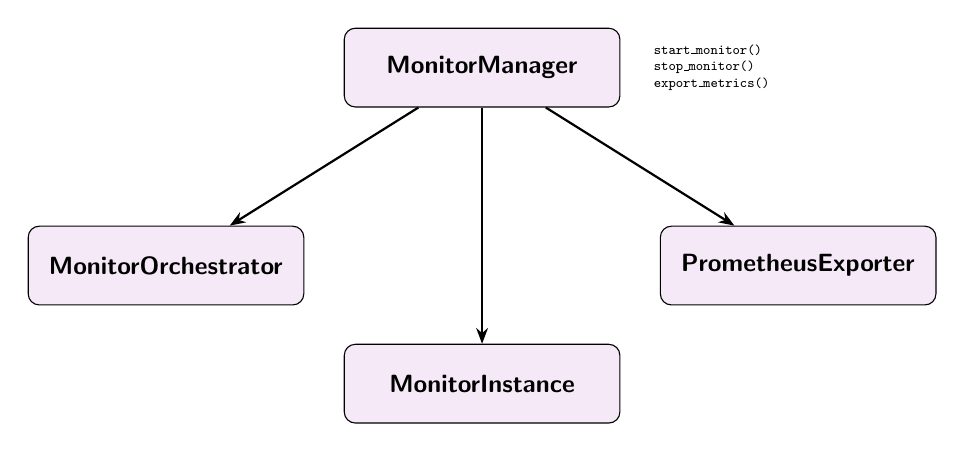
\begin{tikzpicture}[
    node distance=1cm and 1.5cm,
    class/.style={rectangle, draw, rounded corners, fill=monitorPurple!10, minimum width=3.5cm, minimum height=1cm, font=\sffamily\small},
    method/.style={font=\ttfamily\tiny, align=left},
    arrow/.style={-{Stealth[length=2mm]}, thick}
]

\node[class] (manager) {\textbf{MonitorManager}};
\node[class, below left=1.5cm and 0.5cm of manager] (orchestrator) {\textbf{MonitorOrchestrator}};
\node[class, below right=1.5cm and 0.5cm of manager] (exporter) {\textbf{PrometheusExporter}};
\node[class, below=3cm of manager] (instance) {\textbf{MonitorInstance}};

\draw[arrow] (manager) -- (orchestrator);
\draw[arrow] (manager) -- (exporter);
\draw[arrow] (manager) -- (instance);

% Methods
\node[method, right=0.3cm of manager] {
    start\_monitor()\\
    stop\_monitor()\\
    export\_metrics()
};

\end{tikzpicture}
\caption{Monitor Module Class Structure}
\label{fig:monitor-module}
\end{figure}

\subsubsection{MonitorManager}

The \texttt{MonitorManager} orchestrates the complete monitoring lifecycle:

\begin{itemize}
    \item Loading monitor recipes
    \item Resolving target endpoints through service discovery
    \item Generating Prometheus configuration files
    \item Deploying Prometheus as a SLURM job
    \item Managing monitor state persistence
    \item Coordinating metrics export
\end{itemize}

\subsubsection{MonitorOrchestrator}

The \texttt{MonitorOrchestrator} handles Prometheus deployment:

\begin{itemize}
    \item Building SBATCH scripts for Prometheus containers
    \item Managing Apptainer container lifecycle
    \item Generating \texttt{prometheus.yml} configuration
    \item Setting up bind mounts for configuration and data directories
\end{itemize}

\subsubsection{PrometheusExporter}

The \texttt{PrometheusExporter} class provides metrics export functionality:

\begin{itemize}
    \item Querying Prometheus HTTP API for instant and range queries
    \item Service-specific metric selection (e.g., vLLM metrics)
    \item Export to JSON and CSV formats
    \item Common system metrics (CPU, memory, HTTP)
\end{itemize}

\subsection{Target Resolution}

The monitor module automatically resolves targets using service discovery:

\begin{lstlisting}[language=python, caption={Target Resolution Logic}]
def _resolve_targets(self, recipe, targets, job_ids):
    resolved = {}
    
    # Use service discovery
    service_name = recipe.service_name
    discover_info = read_discover_info(service_name)
    
    node = discover_info.get("node")
    ports = discover_info.get("ports", [])
    
    for target in targets:
        port = target.port
        resolved[target.name] = f"{node}:{port}"
    
    return resolved
\end{lstlisting}

\subsection{Prometheus Configuration Generation}

The orchestrator dynamically generates Prometheus configuration:

\begin{lstlisting}[language=yaml, caption={Generated prometheus.yml}]
global:
  scrape_interval: 15s
  evaluation_interval: 15s

scrape_configs:
  - job_name: vllm-metrics
    static_configs:
      - targets: ["mel2013:8000"]
    metrics_path: /metrics
    scrape_interval: 15s
\end{lstlisting}

\subsection{Metrics Export}

The framework supports exporting collected metrics to portable formats:

\begin{lstlisting}[language=bash, caption={Metrics Export Commands}]
# Export instant metrics snapshot
python -m src.monitor export --id abc123 --format json

# Export time-range metrics to CSV
python -m src.monitor export --id abc123 --format csv --type range \
    --start "2025-12-02T10:00:00Z" --end "2025-12-02T11:00:00Z"
\end{lstlisting}

Service-specific metrics are automatically selected based on the monitored service:

\begin{table}[H]
\centering
\caption{vLLM-Specific Prometheus Metrics}
\begin{tabular}{ll}
\toprule
\textbf{Metric} & \textbf{Description} \\
\midrule
\texttt{vllm\_requests\_total} & Total number of requests \\
\texttt{vllm\_request\_duration\_seconds} & Request duration \\
\texttt{vllm\_time\_to\_first\_token\_seconds} & Time to first token \\
\texttt{vllm\_num\_requests\_running} & Running requests \\
\texttt{vllm\_gpu\_cache\_usage\_perc} & GPU cache usage \\
\bottomrule
\end{tabular}
\end{table}

%==============================================================================
\section{Client Module}
%==============================================================================

The Client Module executes benchmarks against deployed AI services, collecting performance metrics and generating reports.

\subsection{Module Architecture}

\begin{figure}[H]
\centering
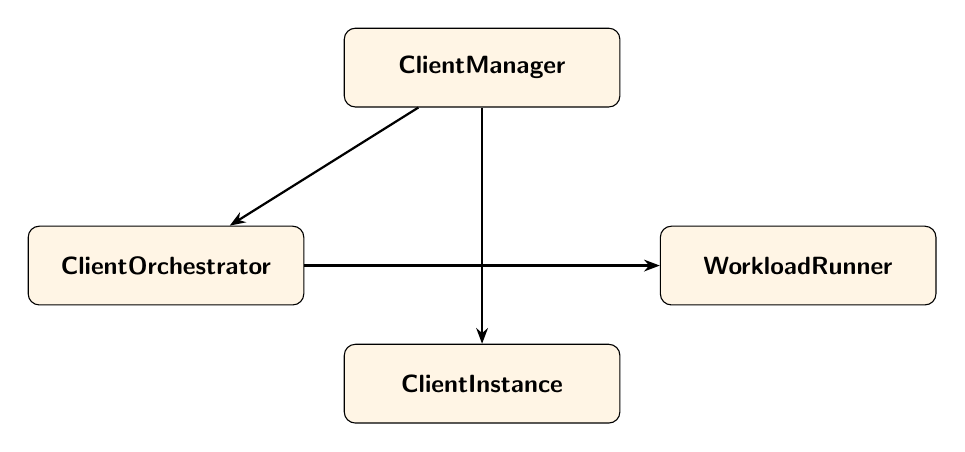
\begin{tikzpicture}[
    node distance=1cm and 1.5cm,
    class/.style={rectangle, draw, rounded corners, fill=clientOrange!10, minimum width=3.5cm, minimum height=1cm, font=\sffamily\small},
    arrow/.style={-{Stealth[length=2mm]}, thick}
]

\node[class] (manager) {\textbf{ClientManager}};
\node[class, below left=1.5cm and 0.5cm of manager] (orchestrator) {\textbf{ClientOrchestrator}};
\node[class, below right=1.5cm and 0.5cm of manager] (runner) {\textbf{WorkloadRunner}};
\node[class, below=3cm of manager] (instance) {\textbf{ClientInstance}};

\draw[arrow] (manager) -- (orchestrator);
\draw[arrow] (manager) -- (instance);
\draw[arrow] (orchestrator) -- (runner);

\end{tikzpicture}
\caption{Client Module Class Structure}
\label{fig:client-module}
\end{figure}

\subsection{Workload Patterns}

The framework supports two workload patterns:

\subsubsection{Closed-Loop Pattern}

Simulates real users with think time between requests:

\begin{lstlisting}[language=yaml]
workload:
  pattern: closed-loop
  concurrent_users: 10
  think_time_ms: 500      # 500ms delay between requests
  requests_per_user: 100
  duration_seconds: 300
\end{lstlisting}

\subsubsection{Open-Loop Pattern}

Generates requests at a fixed rate regardless of response times:

\begin{lstlisting}[language=yaml]
workload:
  pattern: open-loop
  requests_per_second: 50
  duration_seconds: 300
\end{lstlisting}

\subsection{WorkloadRunner}

The \texttt{WorkloadRunner} class executes the actual benchmark:

\begin{itemize}
    \item Makes HTTP requests to the target endpoint
    \item Measures latency for each request
    \item Tracks success/failure rates
    \item Computes aggregate statistics
\end{itemize}

\subsection{Collected Metrics}

\begin{table}[H]
\centering
\caption{Benchmark Output Metrics}
\begin{tabular}{ll}
\toprule
\textbf{Metric} & \textbf{Description} \\
\midrule
\texttt{total\_requests} & Total requests made \\
\texttt{successes} & Successful requests (2xx status) \\
\texttt{errors} & Failed requests \\
\texttt{avg\_latency\_ms} & Average latency \\
\texttt{min\_latency\_ms} & Minimum latency \\
\texttt{max\_latency\_ms} & Maximum latency \\
\texttt{throughput\_req\_per\_sec} & Requests per second \\
\bottomrule
\end{tabular}
\end{table}

%==============================================================================
\section{Recipe System}
%==============================================================================

The recipe system provides a declarative approach to defining deployments, making configurations version-controllable and reproducible.

\subsection{Recipe Types}

\begin{table}[H]
\centering
\caption{Recipe Types and Locations}
\begin{tabular}{lll}
\toprule
\textbf{Type} & \textbf{Directory} & \textbf{Purpose} \\
\midrule
Server & \texttt{recipes/servers/} & AI service deployment \\
Monitor & \texttt{recipes/monitors/} & Prometheus monitoring \\
Client & \texttt{recipes/clients/} & Benchmark workloads \\
\bottomrule
\end{tabular}
\end{table}

\subsection{Recipe Linking}

All recipes for the same service share the \texttt{service\_name} field, enabling automatic discovery and connection between components. This design choice was made to:

\begin{itemize}
    \item Eliminate manual endpoint configuration
    \item Enable one-command deployment workflows
    \item Reduce human error in multi-component setups
\end{itemize}

\subsection{Resource Specification}

Resources are specified consistently across all recipe types:

\begin{lstlisting}[language=yaml]
orchestration:
  resources:
    partition: gpu        # SLURM partition
    cpu_cores: 8          # CPUs per task
    memory_gb: 64         # Memory allocation
    gpu_count: 1          # GPU count (0 for CPU-only)
    time_limit: "04:00:00"  # Job time limit
\end{lstlisting}

%==============================================================================
\section{Design Decisions}
%==============================================================================

This section documents key design decisions made during development and their rationale.

\subsection{File-Based Service Discovery}

\textbf{Decision}: Use JSON files in the user's home directory for service discovery instead of a centralized database or service mesh.

\textbf{Rationale}:
\begin{itemize}
    \item \textbf{Simplicity}: No additional infrastructure required
    \item \textbf{Reliability}: Works with shared filesystems standard in HPC environments
    \item \textbf{User Isolation}: Each user has their own discovery namespace
    \item \textbf{Debugging}: Easy to inspect and manually modify if needed
\end{itemize}

\subsection{Manager-Orchestrator Pattern}

\textbf{Decision}: Separate business logic (Manager) from SLURM interaction (Orchestrator).

\textbf{Rationale}:
\begin{itemize}
    \item \textbf{Testability}: Managers can be tested without SLURM
    \item \textbf{Portability}: Orchestrators can be swapped for other schedulers
    \item \textbf{Maintainability}: Clear separation of concerns
\end{itemize}

\subsection{Synchronous Node Wait}

\textbf{Decision}: Block during server deployment until SLURM assigns a node.

\textbf{Rationale}:
\begin{itemize}
    \item Ensures discovery information is complete before returning
    \item Provides immediate feedback on deployment success
    \item Simplifies client/monitor workflows that depend on server endpoints
\end{itemize}

\subsection{Recipe-Based Configuration}

\textbf{Decision}: Use YAML recipes for all configurations instead of CLI flags.

\textbf{Rationale}:
\begin{itemize}
    \item \textbf{Reproducibility}: Recipes can be version-controlled
    \item \textbf{Complexity Management}: Complex configurations are readable
    \item \textbf{Sharing}: Teams can share standardized configurations
\end{itemize}

\subsection{Prometheus for Monitoring}

\textbf{Decision}: Use Prometheus as the monitoring backend.

\textbf{Rationale}:
\begin{itemize}
    \item Industry standard for metrics collection
    \item Native support in vLLM and many AI frameworks
    \item Pull-based model works well with SLURM job discovery
    \item Rich query language (PromQL) for analysis
\end{itemize}

%==============================================================================
\section{Getting Started}
%==============================================================================

This section provides step-by-step instructions for deploying AI-Factories on MeluXina.

\subsection{Prerequisites}

\begin{itemize}
    \item SSH access to MeluXina cluster
    \item SLURM account (e.g., \texttt{p200981})
    \item Python 3.8+ environment
\end{itemize}

\subsection{Initial Setup}

\begin{lstlisting}[language=bash, caption={MeluXina Setup Commands}]
# 1. Connect to MeluXina
ssh <username>@meluxina.lxp.lu

# 2. Request an interactive session
salloc -A p200981 -t 02:00:00 -q dev

# 3. Navigate to the repository
cd /path/to/AI-Factories

# 4. Run the setup script
./setup.sh

# 5. Configure your SLURM account
export SLURM_ACCOUNT=p200981
\end{lstlisting}

\subsection{Basic Workflow}

\begin{lstlisting}[language=bash, caption={Complete Deployment Workflow}]
# Deploy a vLLM server (auto-registers endpoint)
python -m src.server run --recipe vllm-server
# Output: vllm-server:a1b2c3d4 -> JobID 3757043

# Verify service discovery
python -m src.list_services
# Output: vllm: node=mel2013, ports=[8000]

# Start Prometheus monitoring (auto-discovers server)
python -m src.monitor start --recipe vllm-monitor
# Output: Monitor ID: xyz789, Prometheus: http://mel2014:9090

# Run benchmark (auto-discovers server)
python -m src.client run --recipe vllm-simple-test
# Output: Results saved to ./results/

# Cleanup
python -m src.monitor stop-all
python -m src.server stop-all
python -m src.clear_services
\end{lstlisting}

\subsection{Accessing Prometheus UI}

To access the Prometheus web interface from your local machine:

\begin{lstlisting}[language=bash, caption={SSH Tunnel for Prometheus}]
# From your local machine (new terminal)
ssh -L 9090:mel2014:9090 <username>@meluxina.lxp.lu

# Open in browser
# http://localhost:9090
\end{lstlisting}

%==============================================================================
\section{Benchmarking Results}
%==============================================================================

\textit{This section is a placeholder for benchmarking results that will be completed in a future iteration of this report.}

\subsection{Experimental Setup}

\textbf{TODO}: Document the experimental configuration including:
\begin{itemize}
    \item Hardware specifications (GPU model, memory, etc.)
    \item Model configurations tested
    \item Workload parameters
    \item Duration of experiments
\end{itemize}

\subsection{Performance Metrics}

\textbf{TODO}: Present collected metrics including:
\begin{itemize}
    \item Throughput (requests/second)
    \item Latency distribution (p50, p95, p99)
    \item Time to first token
    \item GPU utilization
    \item Memory consumption
\end{itemize}

\subsection{Comparative Analysis}

\textbf{TODO}: Compare performance across:
\begin{itemize}
    \item Different model sizes
    \item Varying concurrency levels
    \item Open-loop vs. closed-loop patterns
\end{itemize}

\subsection{Scalability Evaluation}

\textbf{TODO}: Analyze scaling behavior with:
\begin{itemize}
    \item Increasing number of concurrent users
    \item Different batch sizes
    \item Multi-GPU configurations (if applicable)
\end{itemize}

%==============================================================================
\section{Future Improvements}
%==============================================================================

Based on development experience and user feedback, the following improvements are planned:

\subsection{Short-Term Enhancements}

\begin{itemize}
    \item \textbf{Multi-Node Server Deployment}: Support for distributed inference across multiple nodes using tensor parallelism.
    \item \textbf{Grafana Integration}: Add Grafana dashboards for visualization alongside Prometheus.
    \item \textbf{Alerting}: Configure Prometheus alerting for service health monitoring.
    \item \textbf{Result Aggregation}: Automatic aggregation and comparison of benchmark runs.
\end{itemize}

\subsection{Long-Term Goals}

\begin{itemize}
    \item \textbf{Web Dashboard}: Browser-based UI for monitoring and management.
    \item \textbf{Additional Backends}: Support for other inference servers (TensorRT-LLM, text-generation-inference).
    \item \textbf{CI/CD Integration}: Automated deployment and testing pipelines.
    \item \textbf{Cost Tracking}: Integration with SLURM accounting for resource usage reports.
    \item \textbf{Auto-Scaling}: Dynamic scaling based on request queue depth.
\end{itemize}

%==============================================================================
\section{Conclusion}
%==============================================================================

AI-Factories provides a comprehensive solution for deploying, monitoring, and benchmarking AI inference services on HPC clusters. The framework addresses key challenges in managing containerized AI workloads in SLURM environments through:

\begin{itemize}
    \item A modular architecture with clear separation of concerns
    \item Automatic service discovery that eliminates manual endpoint management
    \item Recipe-based configuration for reproducible deployments
    \item Integrated Prometheus monitoring with automatic target resolution
    \item Flexible benchmarking capabilities with configurable workload patterns
\end{itemize}

The framework has been successfully deployed and tested on the MeluXina supercomputer, demonstrating its effectiveness for managing AI inference workloads in production HPC environments.

%==============================================================================
% References
%==============================================================================
\section*{References}

\begin{enumerate}
    \item vLLM: Easy, Fast, and Cheap LLM Serving. \url{https://github.com/vllm-project/vllm}
    \item Prometheus Monitoring System. \url{https://prometheus.io/}
    \item Apptainer (Singularity) Container Platform. \url{https://apptainer.org/}
    \item SLURM Workload Manager. \url{https://slurm.schedmd.com/}
    \item MeluXina Supercomputer. \url{https://luxprovide.lu/}
\end{enumerate}

\end{document}